\section{Example Model}

\begin{figure*}
\centering
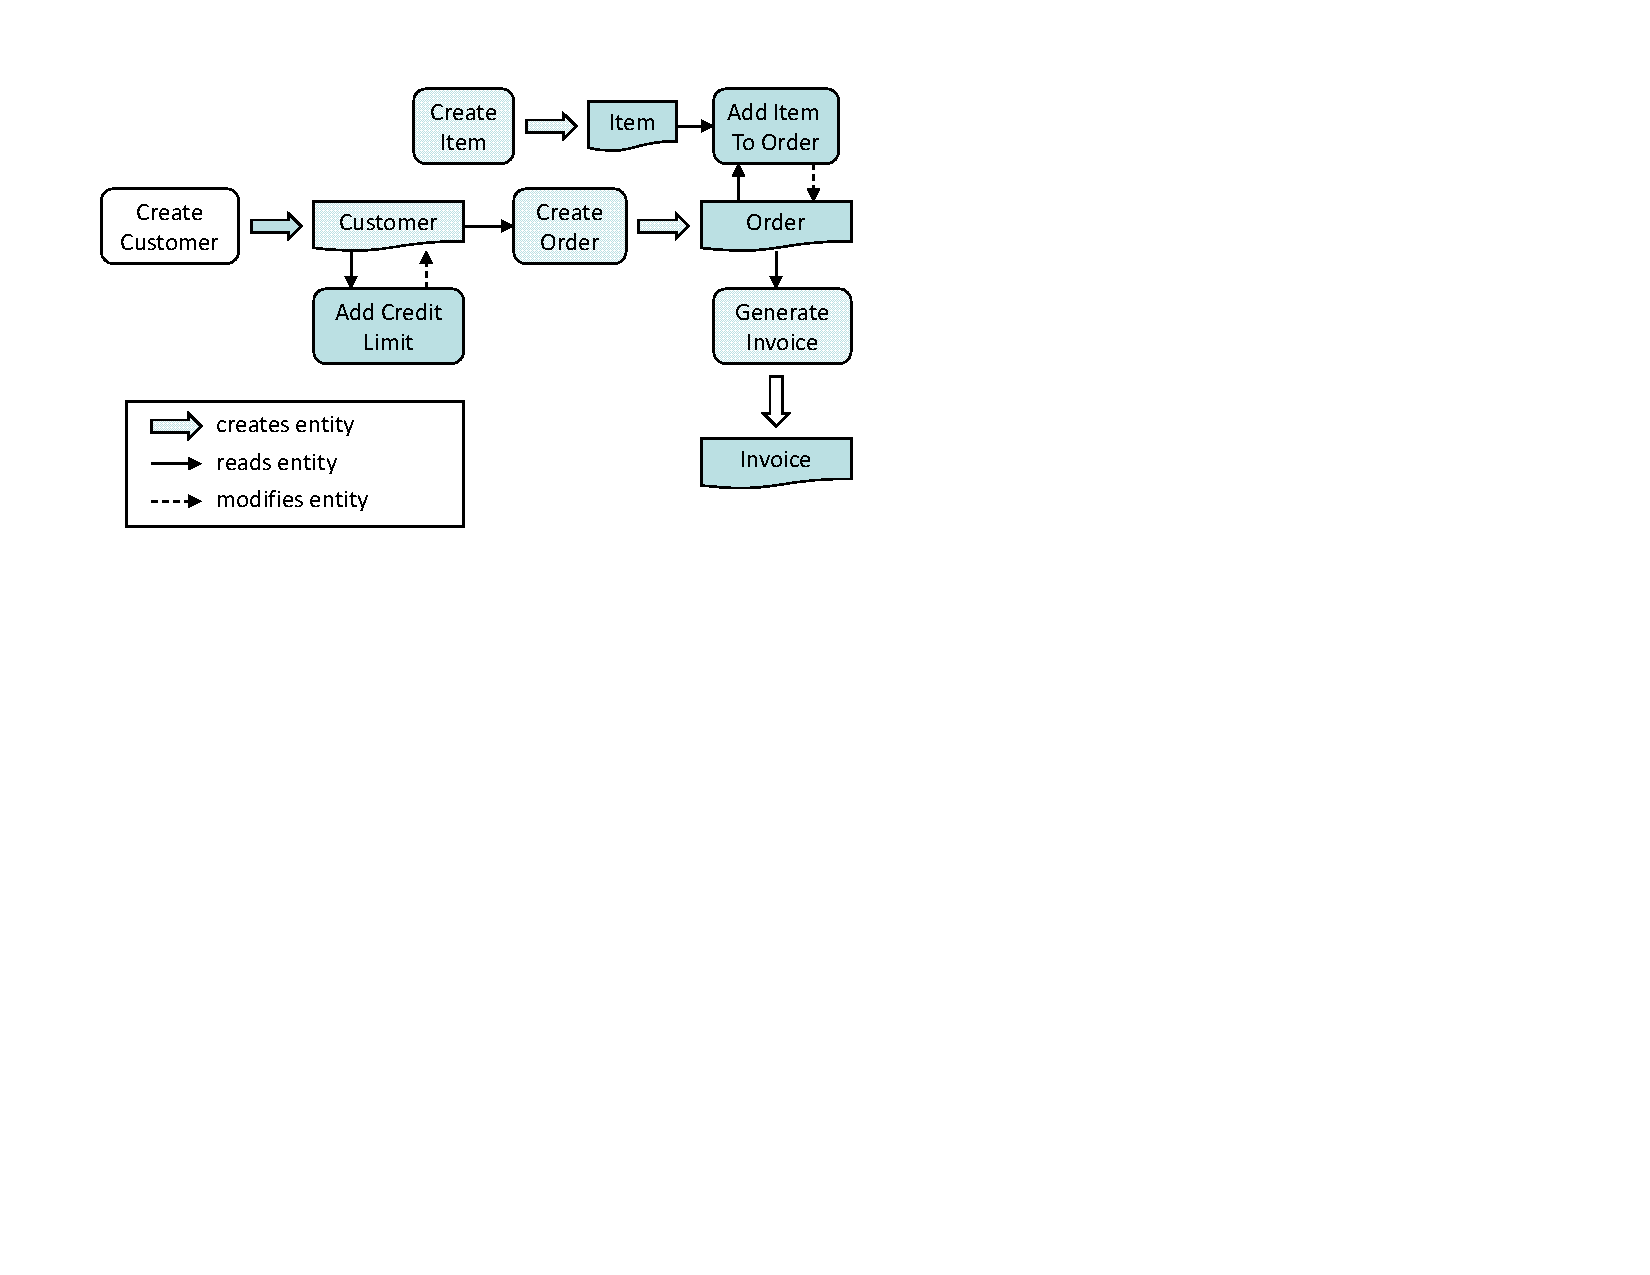
\includegraphics[trim=45 435 40 38,clip,width=7.5in]{figs/appModel.pdf}
\caption{Operations and their interactions with entities of the sample billing application.}
\label{fig:sample-app}
\end{figure*}

We next introduce a sample billing application (along with its operations and rules) that creates 
orders for customers and generates invoices. We use this application as an illustrative example to explain our technique. The 
model includes four entities: \textit{Customer}, \textit{Item}, \textit{Order}, and \textit{Invoice}.
Figure~\ref{fig:sample-app} shows all operations in the application and their interactions (create or modify) with the entities.
For example, the operation \textit{CreateCustomer} creates an instance of \textit{Customer}, whereas
the operation \textit{AddItemToOrder} modifies an \textit{Order} instance by adding a new item to the order.

\begin{table*}[t]
\caption{Formal specification of the business rules in the sample billing application.}
\centering
{\scriptsize
\begin{tabular}{|l|l|l|}
\hline
\multicolumn{1}{|c|}{\small Operation} &
\multicolumn{1}{|c|}{\small Rule Description} &
\multicolumn{1}{|c|}{\small Formal Representation} \\
\hline \hline
CreateCustomer & \textit{Status} of newly created customers should be \textit{Inactive} until they are verified and activated
& TODO \\
\hline
CreateOrder 	 & New orders can be created only for the customers whose \textit{Status} is \textit{Active} 
& TODO \\
\hline
CreateOrder 	 & Orders created in the month of November are eligible for thanksgiving discount of 5\%
& TODO \\
\hline
GenerateInvoice& Invoices cannot be raised for empty orders
& TODO \\
\hline
GenerateInvoice& If the customer belongs to the \textit{NY} \textit{State}, an additional 2\% discount is given while generating invoices
& TODO \\
\hline
\end{tabular}
}
\vspace*{-10pt}
\label{tab:bookstore-rules-spec}
\end{table*}

Table~\ref{tab:bookstore-rules-spec} shows the business rules in each operation. The table provides
both an informal description of each rule and its formal representation expected by our technique.
\note{add formal representation of the rules and describe the rules along with their rule part}